\newpage
\subsection{Incorporating Feedback}
This chapter explains the process of incorporating the feedback from the target group interviews
into the current progress of The DesignAPI. As many changes have been made, only the most impactful
have been highlighted here.

As Mary mentioned that numerous engineers have never been in contact with Figma, a new category was
added to fill this gap.

\textbf{Figmafication} - Focuses on getting developers familiar with using Figma. The
opportunity for this category is to increase the number of engineers actively
incorporating design tools like Figma into their workflows.

Having unified screen breakpoints and keeping responsive components variants close to each other was
mentioned by Peter as a very helpful practice. This resulted in the following two cards being added
to the collection.
%TODO: Add graphics of the two responsiveness cards 

Lastly, Peters example of a situation where a simple Radio-Button would have done the job perfectly,
but instead the designer came up with a much more complex solution was a powerful story.
Identifying parts of the design that would cost much time to implement, but are valuable in contrast
to parts that don't provide enough value and communicating this early to the designer is important.
(vgl 281-389)
It enables the team to deliver value at parts where it actually matters. This sentiment has been
turned into a card as well as a message template.
%TODO: Add graphics of card and message template.

\begin{figure}[H]
    \centering
    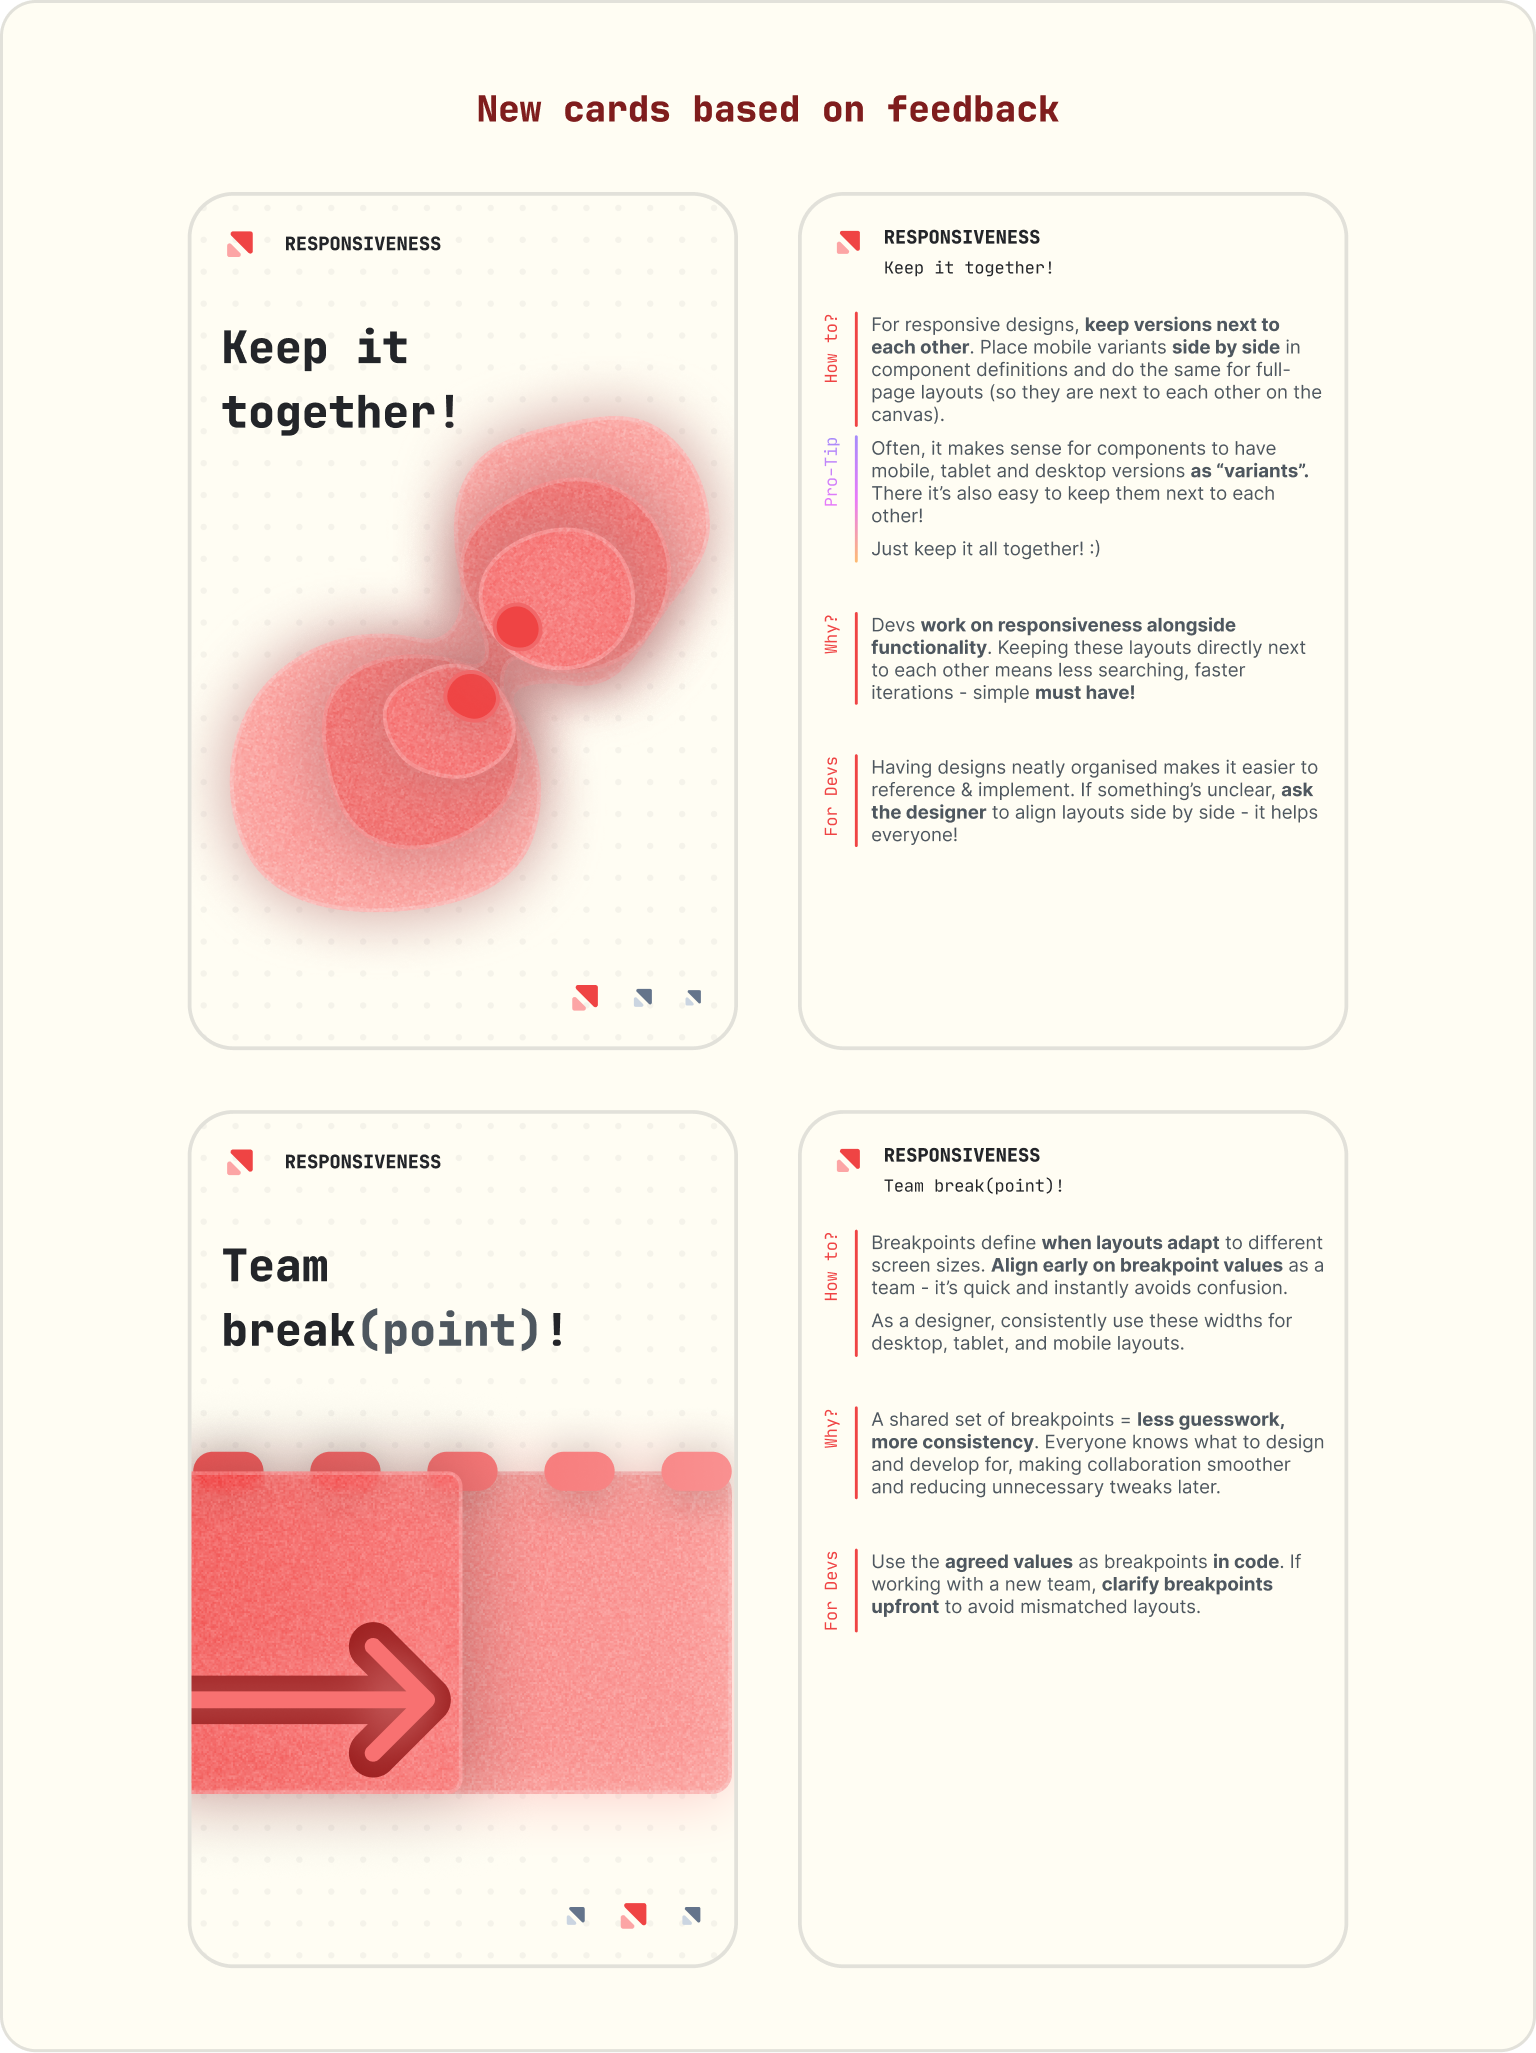
\includegraphics[width=400pt]{Chapter 5/New Cards.png}
    \caption{New cards in the Responsiveness category based on feedback (Source: own illustration)}
\end{figure}

\begin{figure}[H]
    \centering
    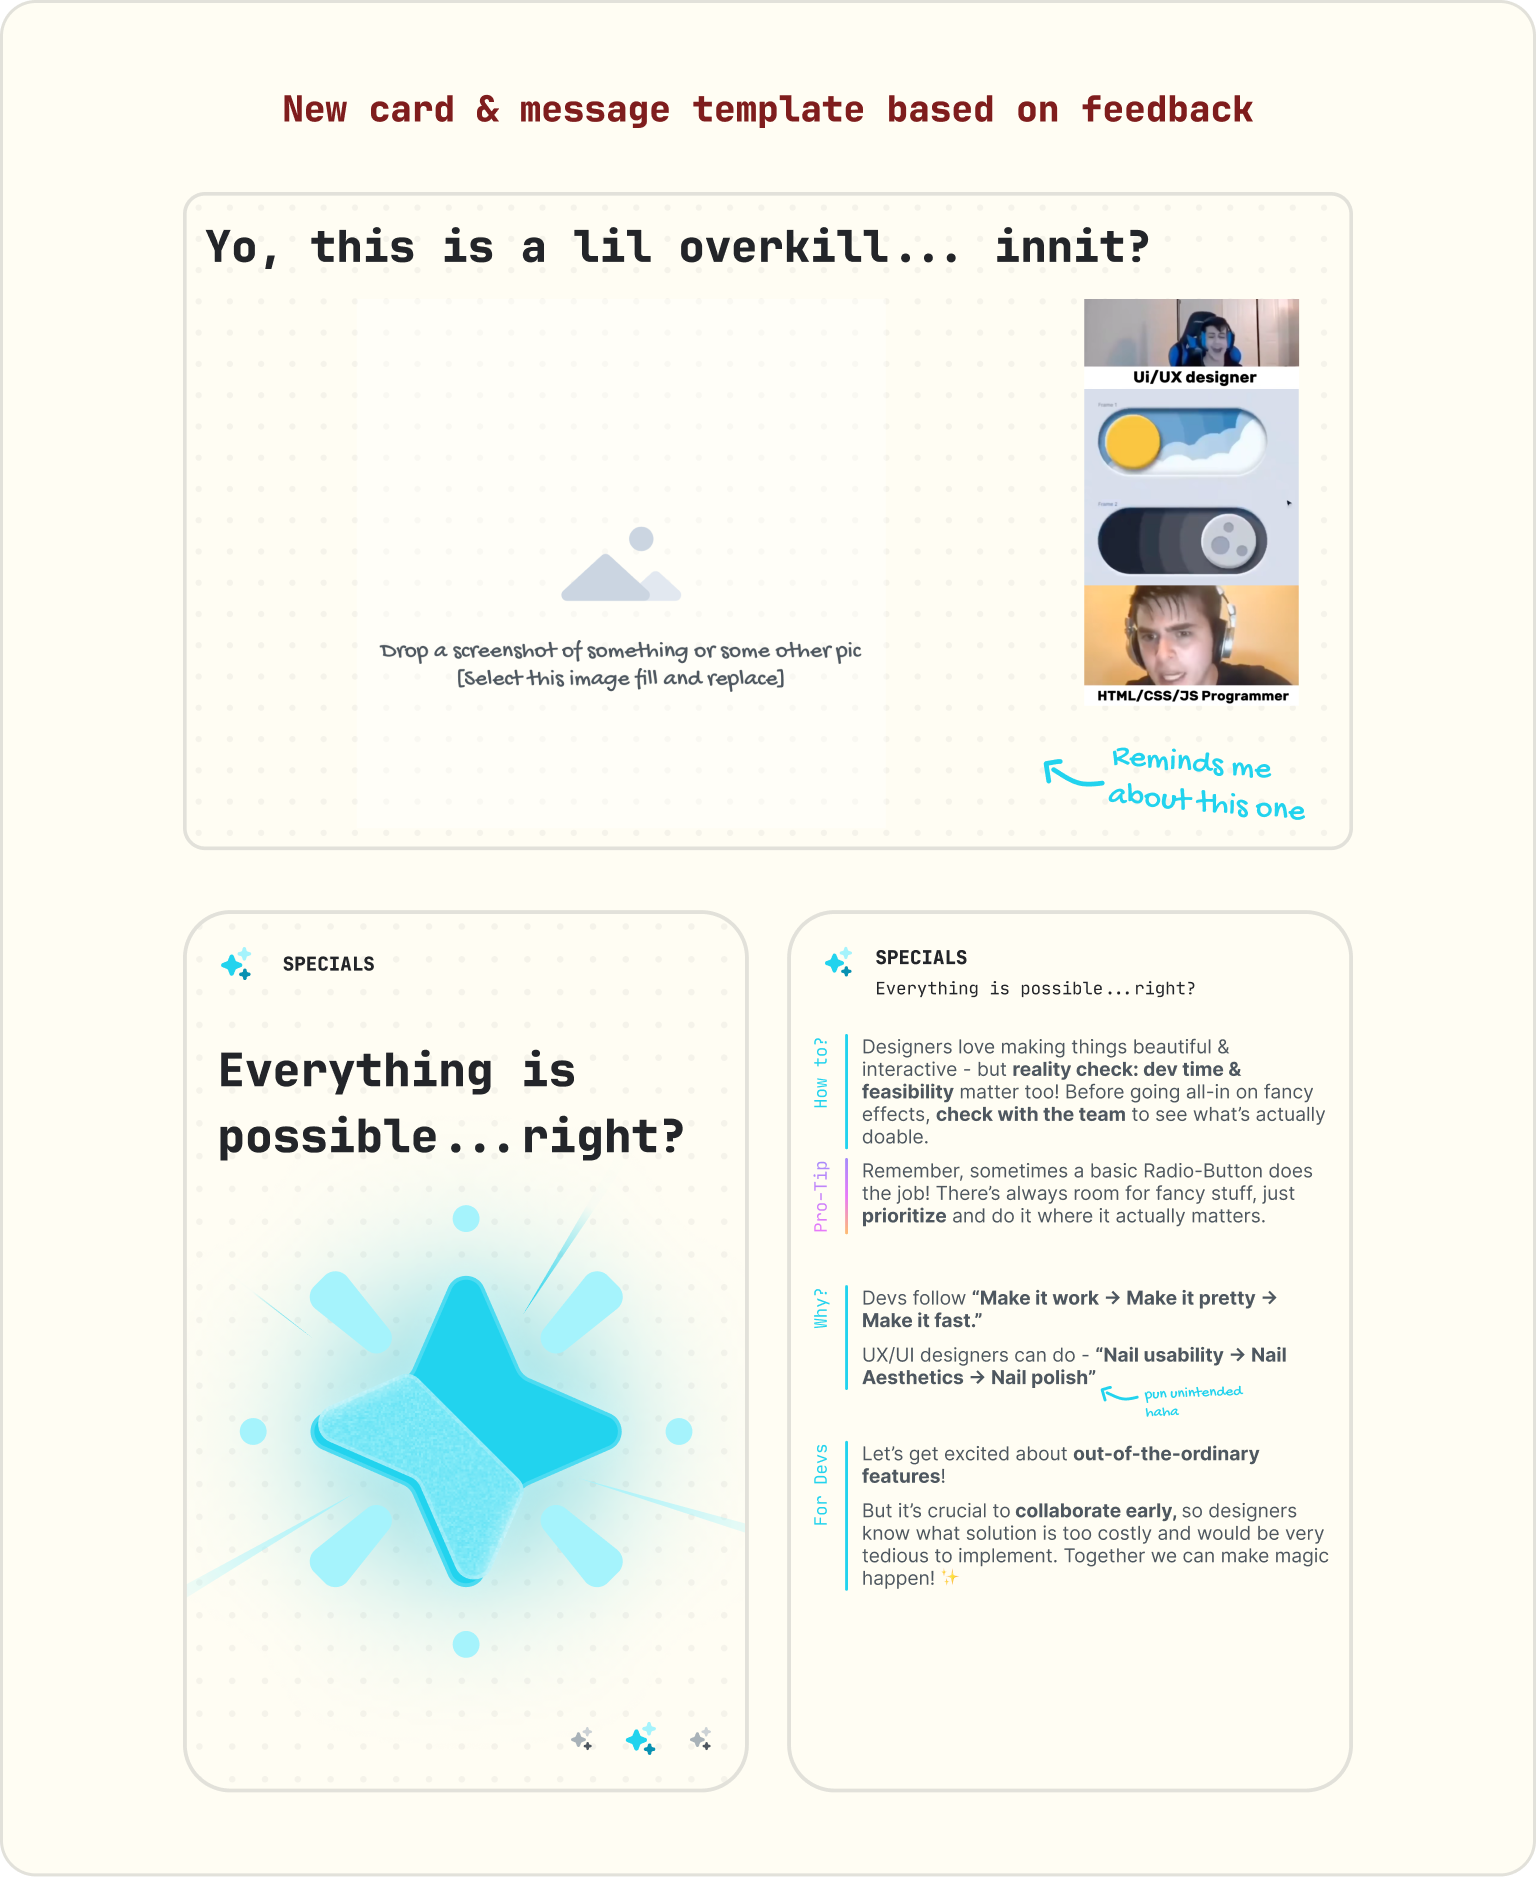
\includegraphics[width=400pt]{Chapter 5/New Card and template.png}
    \caption{New card and message template in the Specials category based on feedback (Source: own illustration)}
\end{figure}
